\documentclass[UTF8]{ctexbeamer}
\usepackage{physics}
\usepackage{amsmath, amssymb, mathtools}
\usepackage{tikz}
\usepackage{mathdots}
\usepackage{yhmath}
\usepackage{cancel}
\usepackage{color}
\usepackage{siunitx}
\usepackage{array}
\usepackage{multirow}
\usepackage{amssymb}
\usepackage{textcomp, gensymb}
\usepackage{tabularx}
\usepackage{extarrows}
\usepackage{booktabs}
\usetikzlibrary{fadings}
\usetikzlibrary{patterns}
\usetikzlibrary{shadows.blur}
\usetikzlibrary{shapes}
\usepackage{listings}
\usepackage{hyperref}

\DeclareMathOperator{\ee}{e}

%Information to be included in the title page:
\title{Hubbard模型的行列式蒙特卡洛模拟}
\author{吴晋渊 18307110155}
\institute{复旦大学物理学系}
\date{2021}

\usetheme{Madrid}

\newcommand{\concept}[1]{\textbf{#1}}
\newcommand{\pair}[1]{\langle #1 \rangle}

\begin{document}

\frame{\titlepage}

\begin{frame}
\frametitle{二维正方晶格Hubbard模型}

Hubbard模型
\begin{equation}
    H = - t\sum_{\pair{\vb*{i}, \vb*{j}}} c^\dagger_{\vb*{i} \sigma} c_{\vb*{j} \sigma} + U \sum_{\vb*{i}} n_{\vb*{i} \uparrow} n_{\vb*{j} \downarrow}
\end{equation}    
\begin{itemize}
    \item 最为著名的强关联电子模型
    \begin{itemize}
        \item 半填充$\Rightarrow$海森堡模型
        \item 掺杂$\Rightarrow$t-J模型:可能的高温超导机制,类似于铜基超导的赝能隙
    \end{itemize}
    \item 不可能解析研究(高维无Bethe ansatz可用,微扰论失效),需要蒙特卡洛模拟
    \begin{itemize}
        \item 量子系统,无离散场构型 $\Rightarrow$ 解决方案:离散路径积分,引入$N$个虚时间点,做Trotter分解,$d$维量子系统=$d+1$维经典统计系统
        \begin{equation}
            \begin{aligned}
                Z &= \trace \ee^{- \beta H} = \sum_{\{ \sigma_1, \ldots, \sigma_N \}} \prod_{n} \mel{\sigma_n}{\ee^{- \Delta \tau H}}{\sigma_{n+1}} \\
                &= \sum_\sigma \prod_n \ee^{- \Delta \tau H[\sigma_n, \sigma_{n+1}]}.
            \end{aligned}
        \end{equation}
        \item 费米子算符无经典对应 $\Rightarrow$ 设法把费米子自由度变成玻色自由度
    \end{itemize}
\end{itemize}

\end{frame}

\begin{frame}
\frametitle{朴素的DQMC}

\concept{离散Hubbard-Stratonovich变换}
\begin{itemize}
    \item 用玻色场取代费米场
    \item 物理图像:用每个格点上的总自旋(或者别的费米算符二次型)取代费米自由度
    \begin{equation}
        \ee^{-\Delta \tau U \sum_{\vb*{i}} (n_{\vb*{i} \uparrow} - 1/2) (n_{\vb*{j} \downarrow} - 1/2)} \simeq \text{const} \times \sum_{s_1, s_2, \ldots, s_n = \pm 1} \ee^{\alpha \sum_{\vb*{i}} s_{\vb*{i}} ({n}_{\vb*{i} \uparrow} - {n}_{\vb*{i} \downarrow})},
    \end{equation}
    \begin{equation}
        N \Delta \tau = \beta, \quad \cosh(\alpha) = \ee^{\Delta \tau U / 2}.
    \end{equation}
    \item 随后可以“积掉”电子自由度,只留下$s_{\vb*{i}, \tau}$
    \begin{equation}
        \trace \ee^{- c^\dagger_i A_{ij} c_j} \ee^{- c^\dagger_i B_{ij} c_j} \cdots = \det(1 + \ee^{- \vb{A}} \ee^{- \vb{B}} \cdots).
    \end{equation}
    \item 这个方法称为\concept{determinant quantum Monte Carlo (DQMC)}
\end{itemize}

\end{frame}

\begin{frame}
\frametitle{朴素的的DQMC}

\begin{itemize}
    \item 定义
    \begin{equation}
        \vb{B}^{\sigma}_{\vb{s}}(\tau) = \ee^{\sigma \alpha \ \mathrm{diag}{\vb{s}_\tau}} \ee^{- \Delta \tau \vb{T}}, \quad \mathbf{B}^\sigma_{\mathbf{s}}\left(\tau_{2}, \tau_{1}\right)=\prod_{n=n_{1}+1}^{n_{2}} \vb{B}^{\sigma}_{\vb{s}}(\tau), 
    \end{equation}
    其中$\sigma = \uparrow, \downarrow \coloneqq \pm 1$,$\vb{s}_{\tau} = [s_{\vb*{i}, \tau}]$,$\vb{s}$为一个$\{s_{\vb*{i}, \tau}\}$构型的简写,$\vb{T}$为一次量子化动能矩阵
    \item 可推导出配分函数(用于计算接受率,DQMC的命名由来)
    \begin{equation}
        Z = \sum_{\vb{s}} Z[\vb{s}], \quad Z[\vb{s}] = \det(1 + \prod_{\sigma=\uparrow, \downarrow} \prod_{n=1}^m \vb{B}_{\vb{s}}^\sigma(\tau) ),
    \end{equation}
    \item 以及等时格林函数(用于计算物理量期望值)
    \begin{equation}
        \vb{G}^\sigma_{\vb*{i} \vb*{j}}(\tau) = \expval*{c_{\vb*{i} \sigma} c^\dagger_{\vb*{j} \sigma}}_\tau = \left(1+\mathbf{B}^\sigma_{\mathbf{s}}(\tau, 0) \mathbf{B}^\sigma_{\mathbf{s}}(\beta, \tau)\right)^{-1}_{\vb*{i}, \vb*{j}}.
    \end{equation}
    \item 计算$\vb{B}^\sigma(\tau_1, \tau_2)$时由于有连乘,需要做数值稳定
\end{itemize}

\end{frame}

\begin{frame}
\frametitle{朴素的DQMC}

\begin{center}
    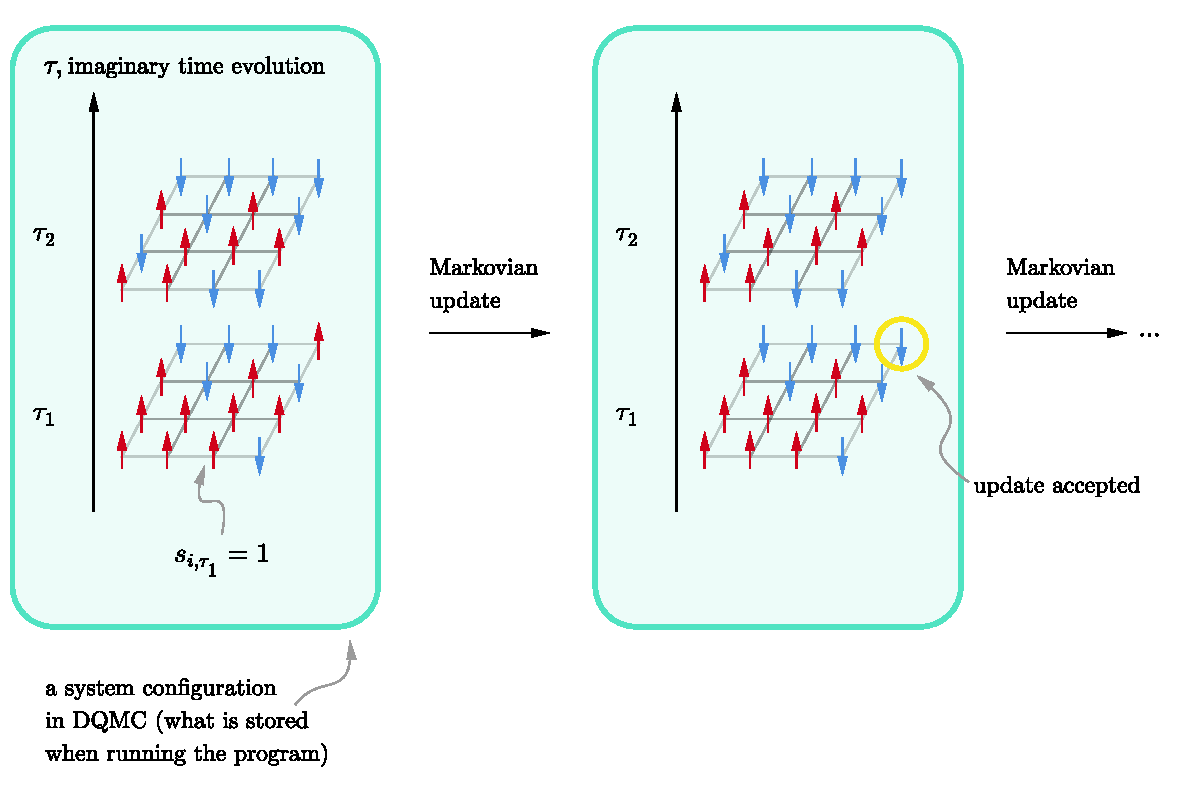
\includegraphics[width=\textwidth]{naive-dqmc.pdf}
\end{center}

\end{frame}

\begin{frame}
\frametitle{基于格林函数的DQMC}

\begin{itemize}
    \item 朴素DQMC性能开销大头:$\vb{B}(\tau_1, \tau_2)$矩阵连乘
    \item 虚时间点$\tau$,空间格点$\vb*{i}$处发生一次更新,则$\vb{B}$矩阵只有如下变化:
    \begin{equation}
        \mathbf{B}^\sigma_{\mathbf{s}^{\prime}}(\tau)=\left(1+\vb{\Delta}^{\vb*{i}, \sigma}\right) \mathbf{B}^\sigma_{\mathbf{s}}(\tau),
    \end{equation}
    其中$\vb{\Delta}^{\vb*{i}, \sigma}$对角,除了$\vb*{i}$号元素为$\ee^{-2 \sigma \alpha s_{\vb*{i}, \tau}} - 1$外其余为零
    \item 可以手动推导出
    \begin{equation}
        R = \prod_{\sigma = \uparrow, \downarrow} \underbrace{\det(1 + \vb{\Delta}^{\vb*{i}, \sigma} (1 - \vb{G}^\sigma_{\vb{s}}(\tau)))}_{R^\sigma},
        \label{eq:accept-rate}
    \end{equation}   
    \begin{equation}
        \vb{G}^\sigma_{\vb{s}'}(\tau) = \vb{G}^\sigma_{\vb{s}}(\tau) - \frac{1}{R^\sigma} \vb{G}^\sigma_{\vb{s}}(\tau) \vb{\Delta}^{\vb*{i}, \sigma} (1 - \vb{G}^\sigma_{\vb{s}}(\tau)).
        \label{eq:green-function-update}
    \end{equation}
    \item 接受率的计算和格林函数的更新其实无需$\vb{B}$矩阵!
    \item 可以将格林函数作为system configuration的一部分,初始化时从$\vb{s}$计算一次,之后似乎不必再计算任何$\vb{B}$矩阵连乘
\end{itemize}

\end{frame}

\begin{frame}
\frametitle{朴素DQMC}

物理量期望值为
\begin{equation}
    \expval*{O} = \sum_{\vb{s}} p(\vb{s}) \expval*{O}_{\vb{s}},
\end{equation}    
$p(\vb{s})$通过蒙特卡洛采样,而$\expval*{O}_{\vb{s}}$遵从Wick定理

\begin{itemize}
    \item 双占据:
    \begin{equation}
        \expval*{n_{\vb*{i} \uparrow} n_{\vb*{i} \downarrow}}_{\vb{s}} = (1 - \expval*{c_{\vb*{i} \uparrow} c^\dagger_{\vb*{i} \uparrow}}_{\vb{s}})  (1 - \expval*{c_{\vb*{i} \downarrow} c^\dagger_{\vb*{i} \downarrow}}_{\vb{s}}).
    \end{equation}
    \item 磁化关联函数:
    \begin{equation}
        \begin{aligned}
            \expval*{s^z_{\vb*{i}} s^z_{\vb*{j}}}_{\vb{s}} &= \frac{1}{4} \expval*{(c^\dagger_{\vb*{i} \uparrow} c_{\vb*{i} \uparrow} - c^\dagger_{\vb*{i} \downarrow} c_{\vb*{i} \downarrow}) ((c^\dagger_{\vb*{j} \uparrow} c_{\vb*{j} \uparrow} - c^\dagger_{\vb*{j} \downarrow} c_{\vb*{j} \downarrow}))}_{\vb{s}} \\
            &= \frac{1}{4} (\expval*{c^\dagger_{\vb*{i} \uparrow} c_{\vb*{i} \uparrow}}_{\vb{s}} \expval*{c^\dagger_{\vb*{j} \uparrow} c_{\vb*{j} \uparrow}}_{\vb{s}}
            + \expval*{c^\dagger_{\vb*{i} \downarrow} c_{\vb*{i} \downarrow}}_{\vb{s}} \expval*{c^\dagger_{\vb*{j} \downarrow} c_{\vb*{j} \downarrow}}_{\vb{s}} \\
            &\quad \  + \expval*{c^\dagger_{\vb*{i} \uparrow} c_{\vb*{j} \uparrow}}_{\vb{s}} \expval*{c_{\vb*{i} \uparrow} c^\dagger_{\vb*{j} \uparrow}}_{\vb{s}} 
            + \expval*{c^\dagger_{\vb*{i} \downarrow} c_{\vb*{j} \downarrow}}_{\vb{s}} \expval*{c_{\vb*{i} \downarrow} c^\dagger_{\vb*{j} \downarrow}}_{\vb{s}} \\
            &\quad \  - \expval*{c^\dagger_{\vb*{i} \downarrow} c_{\vb*{i} \downarrow}}_{\vb{s}} \expval*{c^\dagger_{\vb*{j} \uparrow} c_{\vb*{j} \uparrow}}_{\vb{s}} - \expval*{c^\dagger_{\vb*{j} \downarrow} c_{\vb*{j} \downarrow}}_{\vb{s}} \expval*{c^\dagger_{\vb*{i} \uparrow} c_{\vb*{i} \uparrow}}_{\vb{s}} ).
        \end{aligned}
    \end{equation}
\end{itemize}

\end{frame}

\begin{frame}
\frametitle{基于格林函数的DQMC}

算法纲要:
\begin{itemize}
    \item 系统构型:$\vb{s}$,目前所处的虚时间点$\tau$,$\tau$处的格林函数$\vb{G}^\sigma$
    \item 初始化:初始$s_{\vb*{i}, \tau}$构型,计算各虚时间点的格林函数
    \item 给定$\tau$,翻转$s_{\vb*{i}, \tau}$:接受率为\eqref{eq:accept-rate},如果成功,将$s_{\vb*{i}, \tau}$变更正负号,并且用\eqref{eq:green-function-update}计算新的$\vb{G}^\sigma(\tau)$,$\vb{G}^\sigma \leftarrow \vb{G}^\sigma_{\vb{s}'}(\tau)$
    \item 已经完成$\tau$点处全部格点的翻转,使用
    \begin{equation}
        \vb{G}^\sigma(\tau + \Delta \tau) = \vb{B}^\sigma(\tau + \Delta \tau) \vb{G}^\sigma(\tau) \vb{B}^\sigma(\tau + \Delta \tau)^{-1}
    \end{equation}
    从$\tau$点转移到$\tau \pm \Delta \tau$点,$\vb{G}^\sigma \leftarrow \vb{G}^\sigma(\tau \pm \Delta \tau)$,$\tau \leftarrow \tau \pm \Delta \tau$,然后去翻转新的$\tau$处的$s_{\vb*{i}, \tau}$
    \item 一个sweep:
\end{itemize}

\begin{center}
    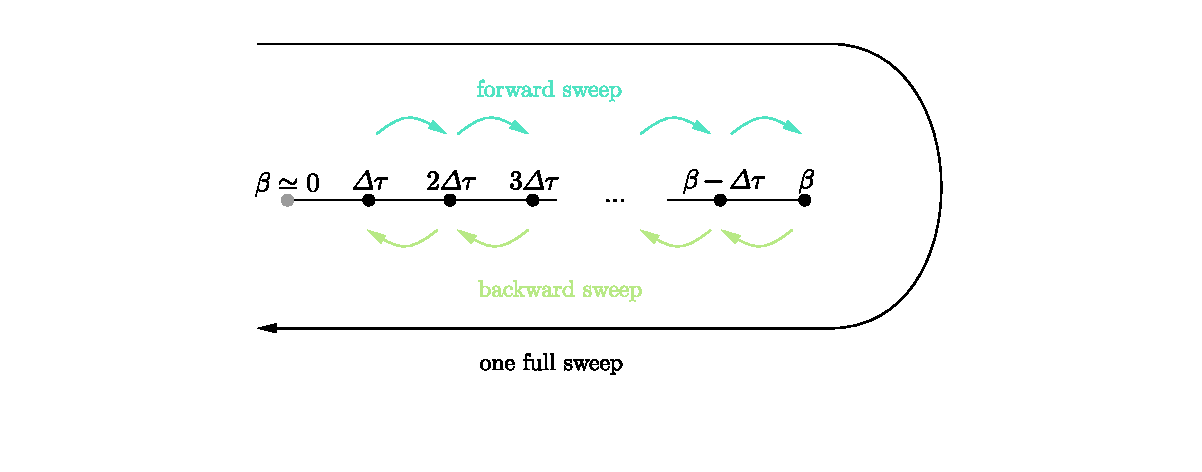
\includegraphics[width=0.7\textwidth]{sweeping.pdf}
\end{center}

\end{frame}

\begin{frame}
\frametitle{格林函数DQMC}

进一步的改进:
\begin{itemize}
    \item 通过矩阵乘法更新格林函数会导致矩阵计算误差指数放大
    \begin{itemize}
        \item 隔一定步数仍然需要重新计算格林函数(称为wrap)
    \end{itemize}
    \item 在时间点$\tau$上的更新不会影响别的虚时间点上的$\vb{B}^\sigma(\tau')$
    \begin{itemize}
        \item 将不同虚时间点的$\vb{B}^\sigma(\tau)$保存起来,避免在wrap的时候重复计算
    \end{itemize}
    \item 用$\vb{G}^\sigma(\tau)$算$\vb{G}^\sigma(\tau \pm \Delta \tau)$时需要左乘、右乘$\vb{B}^\sigma$和$(\vb{B}^\sigma)^{-1}$
    \begin{itemize}
        \item 求逆操作耗时长,直接使用
        \begin{equation}
            \vb{B}^\sigma(\tau)^{-1} = \ee^{\Delta \tau \vb{T}} \ee^{-\sigma \alpha \ \mathrm{diag}{\vb{s}_\tau}}
        \end{equation}
        \item $\ee^{\pm \Delta \tau \vb{T}}$计算用时长,$\vb{T}$计算过程中不变,应该预先算好
        \item 左乘、右乘$\ee^{\pm \sigma \alpha\ \mathrm{diag} \vb{s}_\tau}$应使用为对角矩阵优化的矩阵乘法
    \end{itemize}
\end{itemize}

\end{frame}

\begin{frame}
\frametitle{实现细节}

目标:
\begin{itemize}
    \item 模块化、封装:避免全局变量传参数
    \begin{itemize}
        \item 被修改的变量、被调用的函数是非常透明的
        \item 便于调试
    \end{itemize}
    \item 代码复用
    \begin{itemize}
        \item 可以将DQMC代码整合进更大的程序中,如研究Hubbard模型电子和Ising自旋耦合
        \item 便于改动晶格类型
    \end{itemize}
\end{itemize}    

\end{frame}

\begin{frame}
\frametitle{实现细节}

\begin{columns}

\begin{column}{0.58\textwidth}
    将一个DQMC任务中用到的东西打包在一个结构体中,内容包括:
    \begin{itemize}
        \item 模型参数:$t$, $U$, $\beta$,\texttt{lattice}
        \item 问题规模:虚时间点总数$N$(记作\texttt{n\_imtimes}),经过几个虚时间点做wrap(\texttt{n\_wrap})
        \item 预先算好的物理量:$\Delta \tau$, $\alpha$, $\vb{T}$, $\ee^{\Delta \tau \vb{T}}$(记作\texttt{expT}),$\ee^{- \Delta \tau \vb{T}}$(记作\texttt{expmT})
        \item 系统构型,包括$\vb{s}$(辅助场构型),以及$\vb{B}$矩阵
        \item 格林函数$\vb{G}^\sigma(\tau)$不在其中
        \begin{itemize}
            \item 如果要有,那么目前的虚时间点也必须放在结构体\texttt{HubbardDQMC}中,而mutable struct性能不佳
            \item 可以给\texttt{sweep}函数传回调函数来访问$\vb{G}^\sigma$
        \end{itemize}
    \end{itemize}
\end{column}

\begin{column}{0.42\textwidth}
    % 取自hubbard-dqmc\lib.jl
    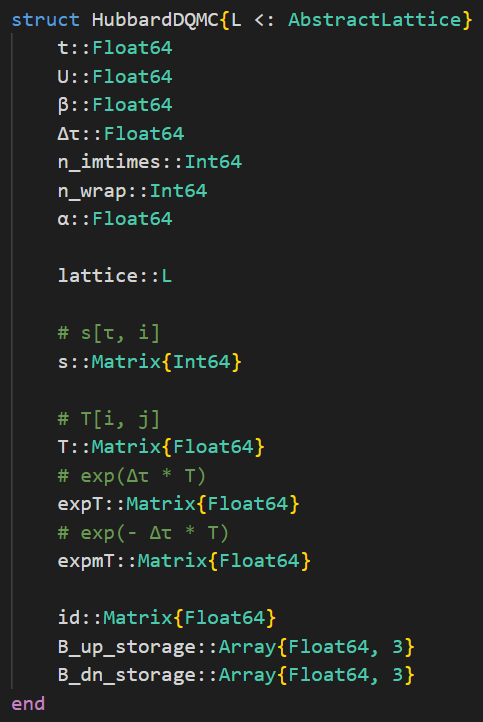
\includegraphics[width=\textwidth]{hubbard-struct.PNG}
\end{column}

\end{columns}    

\end{frame}

\begin{frame}
\frametitle{实现细节}

\begin{columns}

\begin{column}{0.6\textwidth}
    格点信息单独定义,尽可能一般性;从1开始给每个格点编号
    \begin{itemize}
        \item \texttt{site\_list[i, :]}:给出\texttt{i}号格点的坐标
        \item \texttt{inverse\_list[x, y]}:给出$(x, y)$位置处的格点的编号
        \item \texttt{neighbor\_list[i, :]}:给出能够称为\texttt{i}号格点的近邻格点的全部格点
        \item \texttt{neighbor\_list[ineighbor\_list\_indices[1]]}给出\texttt{i}号格点的最近邻格点,将\texttt{1}换成\texttt{2}给出次近邻格点,等等
    \end{itemize}
\end{column}

\begin{column}{0.4\textwidth}
    % hubbard-dqmc\lattice.jl
    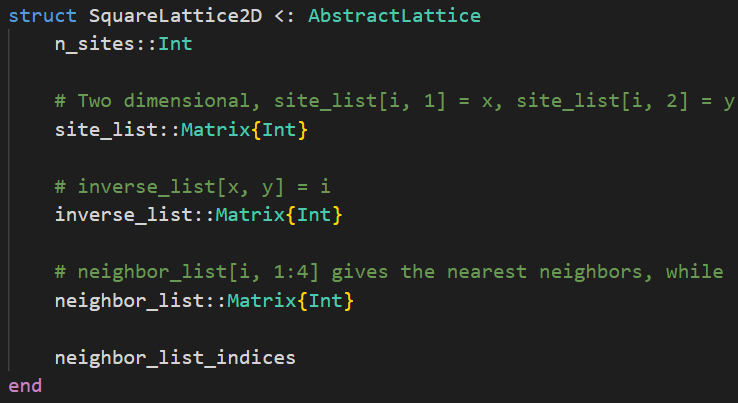
\includegraphics[width=\textwidth]{lattice-def.PNG}
\end{column}

\end{columns}    

\end{frame}

\begin{frame}
\frametitle{实现细节}

格点初始化示例,类似地可以定义三角格子,六角格子等:

% hubbard-dqmc\lattice.jl
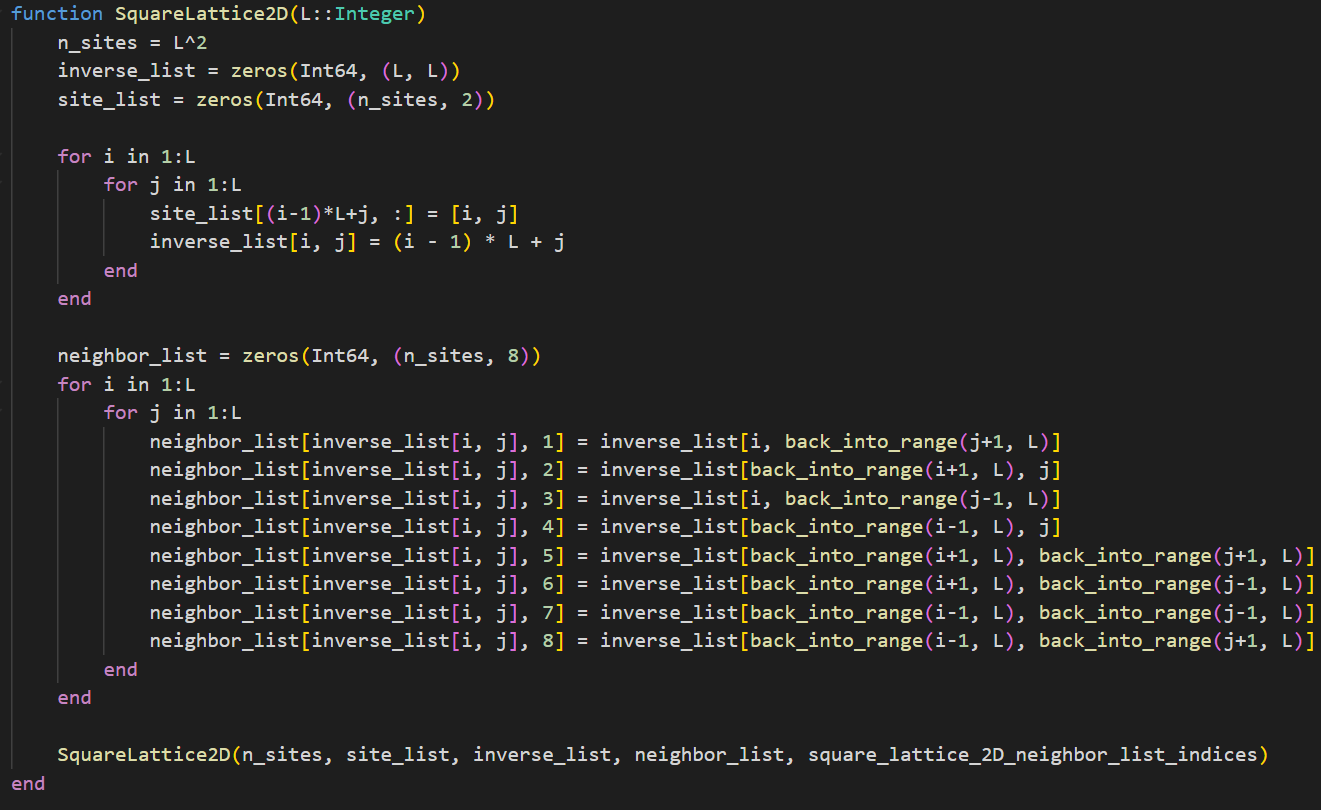
\includegraphics[width=\textwidth]{lattice-initialize.PNG}

\end{frame}

\begin{frame}
\frametitle{实现细节}

计算的中间步骤完全透明,通过\texttt{HubbardDQMC}结构体和其它变量传递数据

\begin{center}
    % hubbard-dqmc\update.jl
    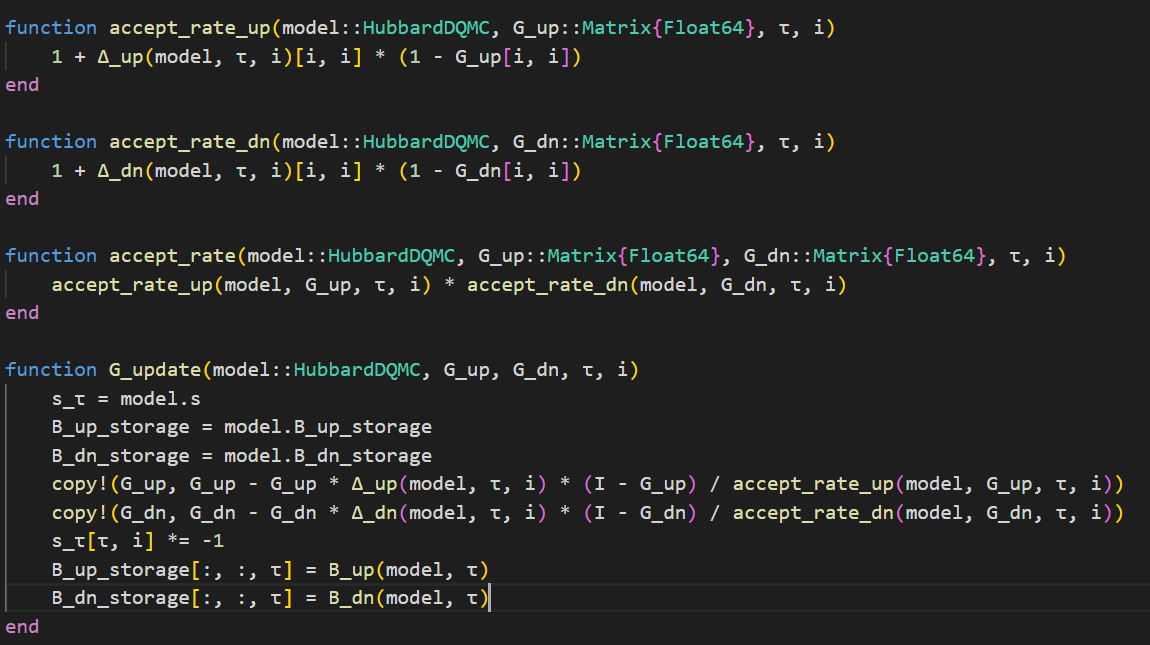
\includegraphics[width=\textwidth]{update-example-1.PNG}
\end{center}

\end{frame}

\begin{frame}
\frametitle{效果}

\begin{columns}[T]

\begin{column}[T]{0.4\textwidth}
    运行界面
    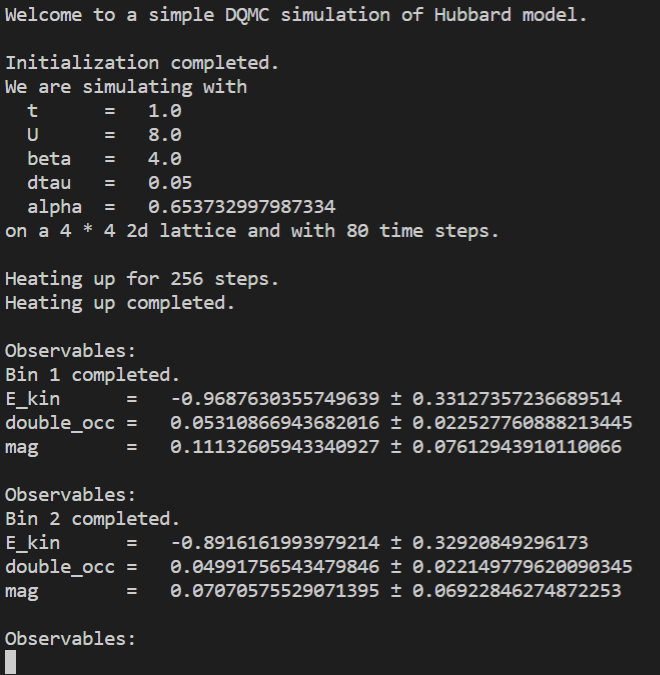
\includegraphics[width=\textwidth]{main-running.PNG}
\end{column}

\begin{column}[T]{0.4\textwidth}
    输出结果
    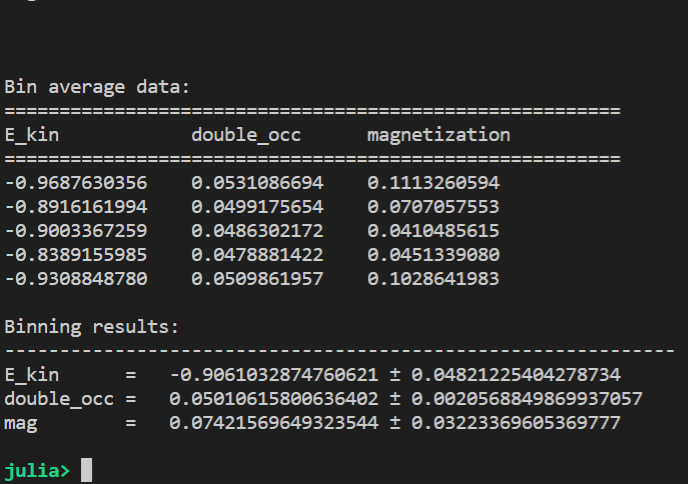
\includegraphics[width=\textwidth]{main-result.PNG}
\end{column}

\end{columns}

\vspace{1em}

计算结果和许霄琰老师的示例代码一致。

\end{frame}

\end{document}